%%%%%%%%%%%%%%%%%%%%%%%%%%%%%%%%%%%%%%%%%
% Professional Newsletter Template
% LaTeX Template
% Version 1.0 (09/03/14)
%
% Created by:
% Bob Kerstetter (https://www.tug.org/texshowcase/) and extensively modified by:
% Vel (vel@latextemplates.com)
% 
% This template has been downloaded from:
% http://www.LaTeXTemplates.com
%
% License:
% CC BY-NC-SA 3.0 (http://creativecommons.org/licenses/by-nc-sa/3.0/)
%
%%%%%%%%%%%%%%%%%%%%%%%%%%%%%%%%%%%%%%%%%

\documentclass[9pt]{extarticle} % The default font size is 10pt; 11pt and 12pt are alternatives

%%%%%%%%%%%%%%%%%%%%%%%%%%%%%%%%%%%%%%%%%
% Professional Newsletter Template
% Structural Definitions File
% Version 1.0 (09/03/14)
%
% Created by:
% Vel (vel@latextemplates.com)
% 
% This file has been downloaded from:
% http://www.LaTeXTemplates.com
%
% License:
% CC BY-NC-SA 3.0 (http://creativecommons.org/licenses/by-nc-sa/3.0/)
%
%%%%%%%%%%%%%%%%%%%%%%%%%%%%%%%%%%%%%%%%%

%----------------------------------------------------------------------------------------
%	REQUIRED PACKAGES
%----------------------------------------------------------------------------------------

\usepackage{listings}
\usepackage{graphicx} % Required for including images
\usepackage{microtype} % Improved typography
\usepackage{multicol} % Used for the two-column layout of the document
\usepackage{booktabs} % Required for nice horizontal rules in tables
\usepackage{wrapfig} % Required for in-line images
\usepackage{float} % Required for forcing figures not to float with the [H] parameter
\usepackage[utf8]{inputenc}
\usepackage{fancyhdr}

%------------------------------------------------
% Fonts

\usepackage{charter} % Use the Charter font as the main document font
\usepackage{courier} % Use the Courier font for \texttt (monospaced) only
\usepackage[T1]{fontenc} % Use T1 font encoding

%------------------------------------------------
% List Separation

\usepackage{enumitem} % Required to customize the list environments
\setlist{noitemsep,nolistsep} % Remove spacing before, after and within lists for a compact look

%------------------------------------------------
% Figure and Table Caption Styles

\usepackage{caption} % Required for changing caption styles
\captionsetup[table]{labelfont={bf,sf},labelsep=period,justification=justified} % Specify the table caption style
\captionsetup[figure]{labelfont={sf,bf},labelsep=period,justification=justified, font=small} % Specify the figure caption style
\setlength{\abovecaptionskip}{10pt} % Whitespace above captions

%------------------------------------------------
% Spacing Between Paragraphs

\makeatletter
\usepackage{parskip}
\setlength{\parskip}{6pt}
\newcommand{\@minipagerestore}{\setlength{\parskip}{6pt}}
\makeatother

%----------------------------------------------------------------------------------------
%	PAGE MARGINS AND SPACINGS
%----------------------------------------------------------------------------------------

\textwidth = 7 in % Text width
\textheight = 10 in % Text height
\oddsidemargin = -18pt % Left side margin on odd pages
\evensidemargin = -18pt % Left side margin on even pages
\topmargin = -36pt % Top margin
\headheight = 0pt % Remove the header by setting its space to 0
\headsep = 0pt % Remove the space between the header and top of the page
\parskip = 2pt % Space between paragraph
\parindent = 0.0in % Paragraph indentation
\pagestyle{empty} % Disable page numbering

%----------------------------------------------------------------------------------------
%	COLORS
%----------------------------------------------------------------------------------------

\usepackage[dvipsnames,svgnames]{xcolor} % Required to specify custom colors

\definecolor{altncolor}{rgb}{.8,0,0} % Dark red
%\definecolor{altncolor}{rgb}{.2,.4,.8} % Dark blue
%\definecolor{altncolor}{rgb}{.84,.16,.16} % Red

\usepackage[colorlinks=true, linkcolor=altncolor, anchorcolor=altncolor, citecolor=altncolor, filecolor=altncolor, menucolor=altncolor, urlcolor=altncolor]{hyperref} % Use the color defined above for all links

%----------------------------------------------------------------------------------------
%	BOX STYLES
%----------------------------------------------------------------------------------------

\usepackage[framemethod=TikZ]{mdframed}% Required for creating boxes
\mdfdefinestyle{sidebar}{
    linecolor=black, % Outer line color
    outerlinewidth=0.5pt, % Outer line width
    roundcorner=0pt, % Amount of corner rounding
    innertopmargin=10pt, % Top margin
    innerbottommargin=10pt, % Bottom margin
    innerrightmargin=10pt, % Right margin
    innerleftmargin=10pt, % Left margin
    backgroundcolor=white, % Box background color
    frametitlebackgroundcolor=white, % Title background color
    frametitlerule=false, % Title rule - true or false
    frametitlerulecolor=white, % Title rule color
    frametitlerulewidth=0.5pt, % Title rule width
    frametitlefont=\Large, % Title heading font specification
    font=\small
}

\mdfdefinestyle{intextbox}{
    linecolor=black, % Outer line color
    outerlinewidth=0.5pt, % Outer line width
    roundcorner=10pt, % Amount of corner rounding
    innertopmargin=7pt, % Top margin
    innerbottommargin=7pt, % Bottom margin
    innerrightmargin=7pt, % Right margin
    innerleftmargin=7pt, % Left margin
    backgroundcolor=white, % Box background color
    frametitlebackgroundcolor=white, % Title background color
    frametitlerule=false, % Title rule - true or false
    frametitlerulecolor=white, % Title rule color
    frametitlerulewidth=0.5pt, % Title rule width
    frametitlefont=\Large % Title heading font specification
}

%----------------------------------------------------------------------------------------
%	HEADING STYLE
%----------------------------------------------------------------------------------------

\newcommand{\heading}[2]{ % Define the \heading command
\vspace{#2} % White space above the heading
{\begin{center}\Large\textbf{#1}\end{center}} % The heading style
\vspace{#2} % White space below the heading
}

\newcommand{\BackToContents}{\hyperlink{contents}{{\small Back to Contents}}} % Define a command for linking back to the contents of the newsletter % Include the document which specifies all packages and structural customizations for this template

\usepackage{amssymb}% http://ctan.org/pkg/amssymb
\usepackage{proof}
\usepackage{pifont}% http://ctan.org/pkg/pifont
\newcommand{\cmark}{\ding{51}}%
\newcommand{\xmark}{\ding{55}}%

\begin{document}

%--------------------------------------------------------------------------------
% HEADER DETAILS
%--------------------------------------------------------------------------------

\pagestyle{fancy}
\fancyhf{}
\chead{segfault@csh.rit.edu}
\rhead{\today}
\lhead{Volume XLVIII Issue \#2}
\addtolength\footskip{-15px}
\cfoot{"You know what would be convenient? If dead bodies could hide 
	themselves." - Holden Lewis (holden)}

%----------------------------------------------------------------------------------------
%	HEADER IMAGE
%----------------------------------------------------------------------------------------

\begin{figure}[H]
\centering\vspace{0.5cm}
\includegraphics[width=0.8\linewidth]{imgs/segfault.png}
\end{figure}

%--------------------------------------------------------------------------------
% HEADER QUOTE
%--------------------------------------------------------------------------------

\vspace{-15px}
\begin{quote}
\centering
\textbf{\textit{It seemed like a good idea at the time}}
\end{quote}
\vspace{10px}

%----------------------------------------------------------------------------------------
%	SIDEBAR - FIRST PAGE
%----------------------------------------------------------------------------------------

\vspace{-0.5cm}\begin{minipage}[t]{.35\linewidth} % Mini page taking up 35% of the actual page
\begin{mdframed}[style=sidebar,frametitle={}] % Sidebar box

%-----------------------------------------------------------

\hypertarget{contents}{\textbf{{\large This week on floor\ldots}}} % \hypertarget provides a label to reference using \hyperlink{label}{link text}
\begin{itemize}
\item \hyperlink{firstnews}{Subtyping}
\end{itemize}

\centerline {\rule{.75\linewidth}{.25pt}} % Horizontal line

%-----------------------------------------------------------

\textbf{Notable Upcoming Events:}
\begin{enumerate}[leftmargin=0.2cm]
\item \textbf{<EVENT NAME>} <DATE + TIME> \\
	<DESCRIPTION>
\\
\item \textbf{<EVENT NAME>} <DATE + TIME> \\
	<DESCRIPTION>
\\
\end{enumerate}

%-----------------------------------------------------------


\textbf{<TITLE>} \\
<SHORT SECTION>
\\

%-----------------------------------------------------------

\captionof*{table}{Voting Results}
\begin{tabular}{lcr}

Vote & Cost & Result \\
\midrule
<NAME> & \$<MONEY> & <STATUS> \\
\bottomrule
\end{tabular}

%-----------------------------------------------------------

\end{mdframed}
\end{minipage}\hfill % End the sidebar mini page 
%
%----------------------------------------------------------------------------------------
%	MAIN BODY - FIRST PAGE
%----------------------------------------------------------------------------------------
%
\begin{minipage}[t]{.61\linewidth} % Mini page taking up 61% of the actual page
\vspace{-0.4cm}
\hypertarget{firstnews}{\heading{Subtyping}{6pt}}

The concept of subtyping is found throughout most programming languages. What it
entails is that if we are given type \textit{A}, then we can defined a narrower
type \textit{B}, such that all values of type \textit{B} are also of type 
\textit{A}. This relationship is written as \textit{B} <: \textit{A}. 
This subtyping relationship is reflexive (\textit{A} <: \textit{A})  and transitive
(\textit{A} <: \textit{B} $\bigwedge$ \textit{B} <: \textit{C} $\rightarrow$
\textit{A} <: \textit{C}). Function subtyping is defined as: \\
\\
\centerline{$\infer{\tau'_a\ \rightarrow\ \tau'_r\ <:\ \tau_a\ \rightarrow\ \tau_r}
	   {\tau_a\ <:\ \tau'_a\ \ \ \tau'_r\ <:\ \tau_r}$}
\\
\textbf{Covariance}: \\
Say for example we have a function of type \textit{Boolean} $\rightarrow$
\textit{Integer} and that \textit{Integer} <: \textit{Double}. This return type
of this function is \textit{Integer} though it can be also be subtyped to return 
types of \textit{Double}. This \textbf{replacement of wider types with narrower
types} is called covariance. Function are covariant in their result types. \\
\\
\centerline{$\infer{boolean\ \rightarrow\ integer\ <:\ boolean \rightarrow\ double}
	   {boolean\ <:\ boolean\ \ \ integer\ <:\ double}$}
\\
\textbf{Contravariance}: \\
Consider the function of type \textit{Double} $\rightarrow$ \textit{Boolean}. We
can use this function anywhere that expects a function of type \textit{integer}
$\rightarrow$ \textit{boolean}. This \textbf{replacement of narrower types with 
wider types} is called contravirance. This is allowed since \textit{integer} <:
\textit{double}.Functions are contravariant in their argument types. \\
\\
\centerline{$\infer{double \rightarrow\ boolean\ <:\ integer\ \rightarrow\ boolean}
	   {integer\ <:\ double\ \ \ boolean\ <:\ boolean}$}
\\
\\
\textbf{Lambda Calculus Example}: \\
$\lambda$ x. \{$l_1$: int, $l_2$: int\}. \{$l_1$: x.$l_2$, $l_2$: x.$l_1$\} \\
$\cdot$ $\vdash$ $\lambda$ x. \{$l_1$: int, $l_2$: int\}. \{$l_1$: x.$l_2$, $l_2$: x.$l_1$\} : \{$l_1$: int, $l_2$: int\} $\rightarrow$ \{$l_1$: int, $l_2$: int\}  \\
\\
S-RCDWIDTH: 
$\infer{\{l_1\ :\ \tau_1,\ ...,\ l_{n+1}\ :\ \tau_{n+1}\}\ <:\ \{l_1\ :\ \tau_1,\ ...,\ l_n\ :\ \tau_n\}}{}$ \\
\\
While this seems complicated, all it does is define a function that takes a record
of size 2 and returns the input record with the elements swapped in it. The type 
rule S-RCDWIDTH gives us the declaration of width subtyping. This rule just says
that records with more fields is a subtype of records with smaller amount of fields,
if all the other fields left are the same type. This function can be subtyped to 
many different types as long as we are contravariance in the argument type and covariance in the result. 

\cmark \{$l_1$: int, $l_2$: int, $l_3$: int\} $\rightarrow$ \{$l_1$: int\} \\
\xmark \{$l_1$: int\} $\rightarrow$ \{$l_1$: int\} \\
\xmark \{$l_1$: int, $l_2$: int\} $\rightarrow$ \{$l_1$: int, $l_2$: int\, $l_3$: int\}  \\
The first one type checks since it is contraviariant in the argument type and
covariant in the result. This is valid since
\{$l_1$: int, $l_2$: int, $l_3$: int\} <: \{$l_1$: int, $l_2$: int\} and 
\{$l_1$: int, $l_2$: int\} <: \{$l_1$: int\}. The other two do not follow the
typing rule S-RCDWIDTH. 

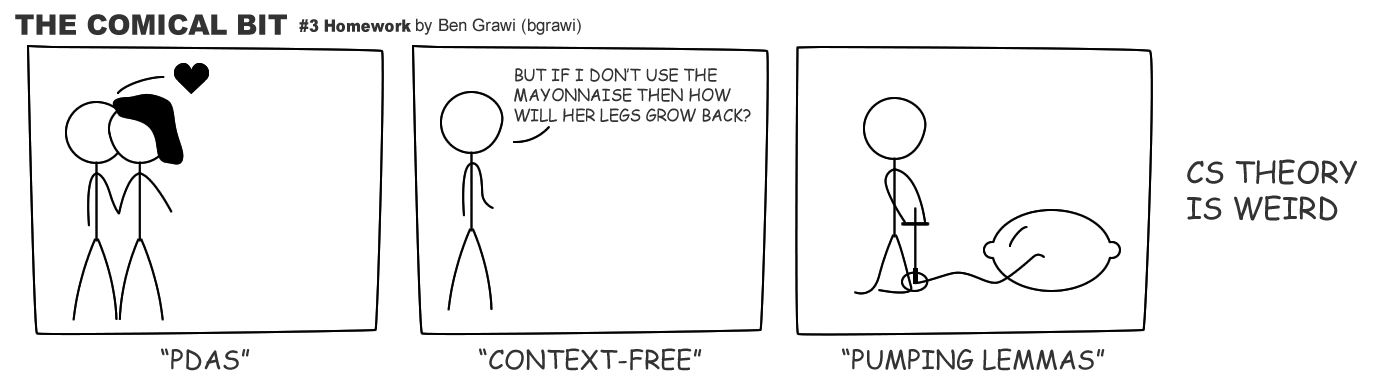
\includegraphics[width=\linewidth]{imgs/cstheory.png} 
\end{minipage} % End the main body - first page mini page

\end{document} 
